% version 1.00, date 19/04/16, auteur Michel Cressant

\documentclass[asi]{picInsa}

%Pour le schéma d'architecture
\usepackage{etex}
\usepackage{tikz}
\usetikzlibrary{shapes,arrows,chains,backgrounds,fit}
%FIN Pour le shéma d'architecture

\DeclareGraphicsRule{*}{pdf}{*}{}
\usepackage{pdfpages}
\usepackage{vocabulaireUnipik}




\setcounter{secnumdepth}{4}
\setcounter{tocdepth}{4}
\newcommand{\ligneMaj}[3] {
	\rowcolor[gray]{0.55} \textbf{\textit{#1}} & #2  &  #3\\
	\hline
}
\newcommand{\ligneSup}[3] {
	\rowcolor[gray]{0.65} |\textunderscore \textbf{\textit{#1}} & #2  &  #3\\
	\hline
}
\newcommand{\ligneMed}[3] {
	\rowcolor[gray]{0.75} \hspace{0.25cm} |\textunderscore #1  & #2 & #3 \\
	\hline
}
\newcommand{\ligneSub}[3] {
	\rowcolor[gray]{0.85}  \hspace{0.5cm} |\textunderscore #1 & #2 & #3\\
	\hline
}
\newcommand{\ligneSubSub}[3] {
	\rowcolor[gray]{0.95}  \hspace{0.75cm} |\textunderscore #1 & #2 & #3\\
	\hline
}
\newcommand{\ligneTache}[3] {
	\hspace{1.00cm} |\textunderscore #1 & #2 & #3\\
	\hline
}
\title{\DCD{}}
\author{\Florian{}, \Kafui{}, \Melissa{}, \Julie{}} 


\titreGeneral{\DCD}
\sousTitreGeneral{\nomEquipe}
\titreAcronyme{\DCDCourt}

\titreDetaille{\DCDCourt\_D\_\nomEquipe\_ l3}
\referenceVersion{\DCDCourt\_D\_\nomEquipe\_\versionPrive}
\auteurs{\Melissa{} \& \Florian{} \& \Michel{} \& \Julie \& \Mathieu \& \Matthieu \& \Kafui}
\destinataires{\nomEquipe}
\resume{Le présent document contient la présentation du \DCD{} \nomEquipe.}
\motsCles{\DCDCourt{}}
\natureDerniereModification{Création}
\modeDiffusionControle{}

\begin{document}

\couverture{}

 \informationsGenerales{}
% version 1.00, date 29/02/16, auteur Michel Cressant
\begin{pagesService}
	\begin{historique}
		% nouvelles versions à rajouter AU-DESSUS en recopiant les lignes suivantes et en les modifiant :
		\unHistorique{1.00}{02/02/2016}{\Michel}{Création}{Toutes}

	\end{historique}

%        \begin{suiviDiffusions}
%
%            % On place ici les diffusions
%        	\unSuivi{1.00}{}{\nomEquipe{}}
%          
%          
%        \end{suiviDiffusions}

%%Signataires
        \begin{signatures}
	   \uneSignature{Vérificateur}{\RRS}{\Matthieu{}}{17/03/2016}{PGPic}
       \uneSignature{Validateur}{\CP{}}{\Sergi}{}{PGPic}
        \end{signatures}
	
	

	
	
\end{pagesService}


\tableofcontents

\setcounter{chapter}{0}


\chapter*{Introduction}
\label{intro}
% version 1.01 Date 24/03/2016	Auteur Mathieu Medici

\section*{Objet}
L'objectif de ce document est de présenter les principes et les procédures nécessaires à la mise en œuvre de la gestion des configurations prévue par la norme \isoNeufMilleUn.

\section*{Définition}

Le présent document établit les règles et la structure de la gestion des configurations qui doivent être suivies pendant toute la durée du \picCourt. Il contient :
\begin{itemize}
\item les règles de nommage;
\item la description des différents référentiels;
\item les règles spécifiques de \nomEquipe{};
\item la description de l'administration des configurations;
\item la description de la maîtrise des documents;
\item la description de la maîtrise des enregistrements;
\item les règles d'archivage.
\end{itemize}



\chapter{Diagramme de package}
\label{diagrammeDePackage}
% version 1.00, date 21/04/16, auteur Michel Cressant

Ce chapitre décrit le diagramme de package. \\

La figure suivante (figure \ref{diagrammeDePackagePng} ) présente le diagramme de package.

\begin{figure}
	\centering
	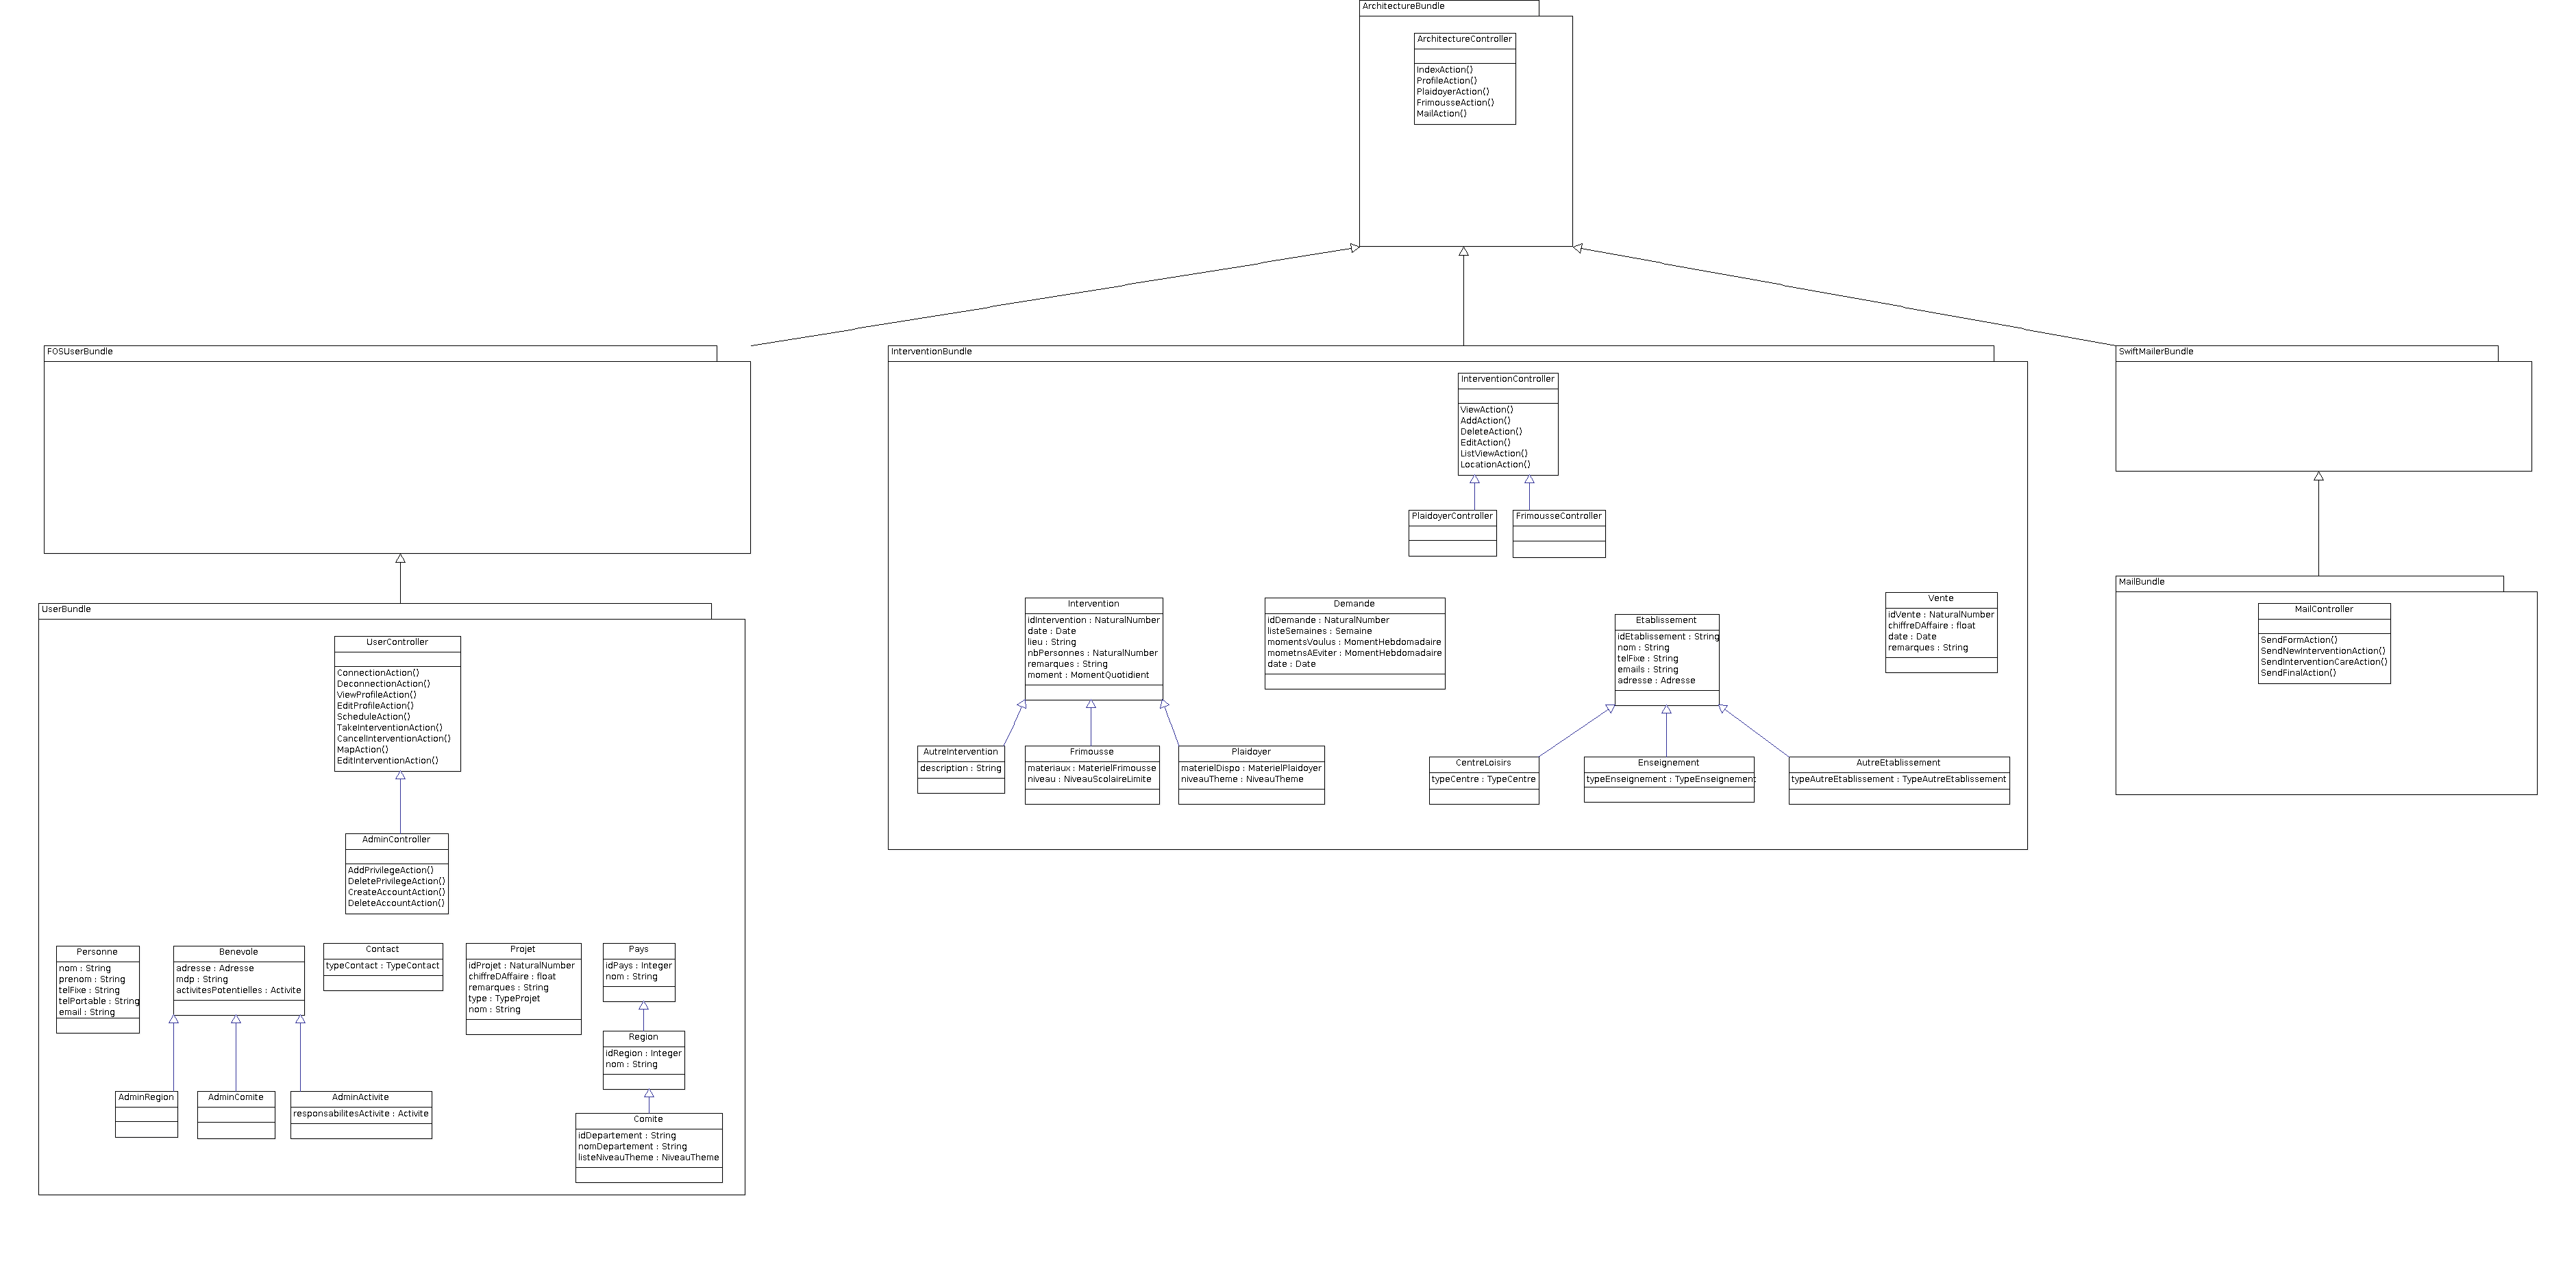
\includegraphics[scale=0.195, angle=90]{images/diagrammePackages/diagrammePackage.png}
	\caption{Diagramme de packages}
	\label{diagrammeDePackagePng}
\end{figure}

\chapter{Carte de navigation}
\label{diagrammeNavigation}
% version 1.00, date 21/04/16, auteur Michel Cressant

Ce chapitre décrit la carte de navigation sous la forme d'un diagramme d'état-transissions. \\

La figure suivante (figure (\ref{carteDeNavigation})) présente la carte de navigation sous la forme d'un diagramme d'état-transissions.

\begin{figure}
	\centering
	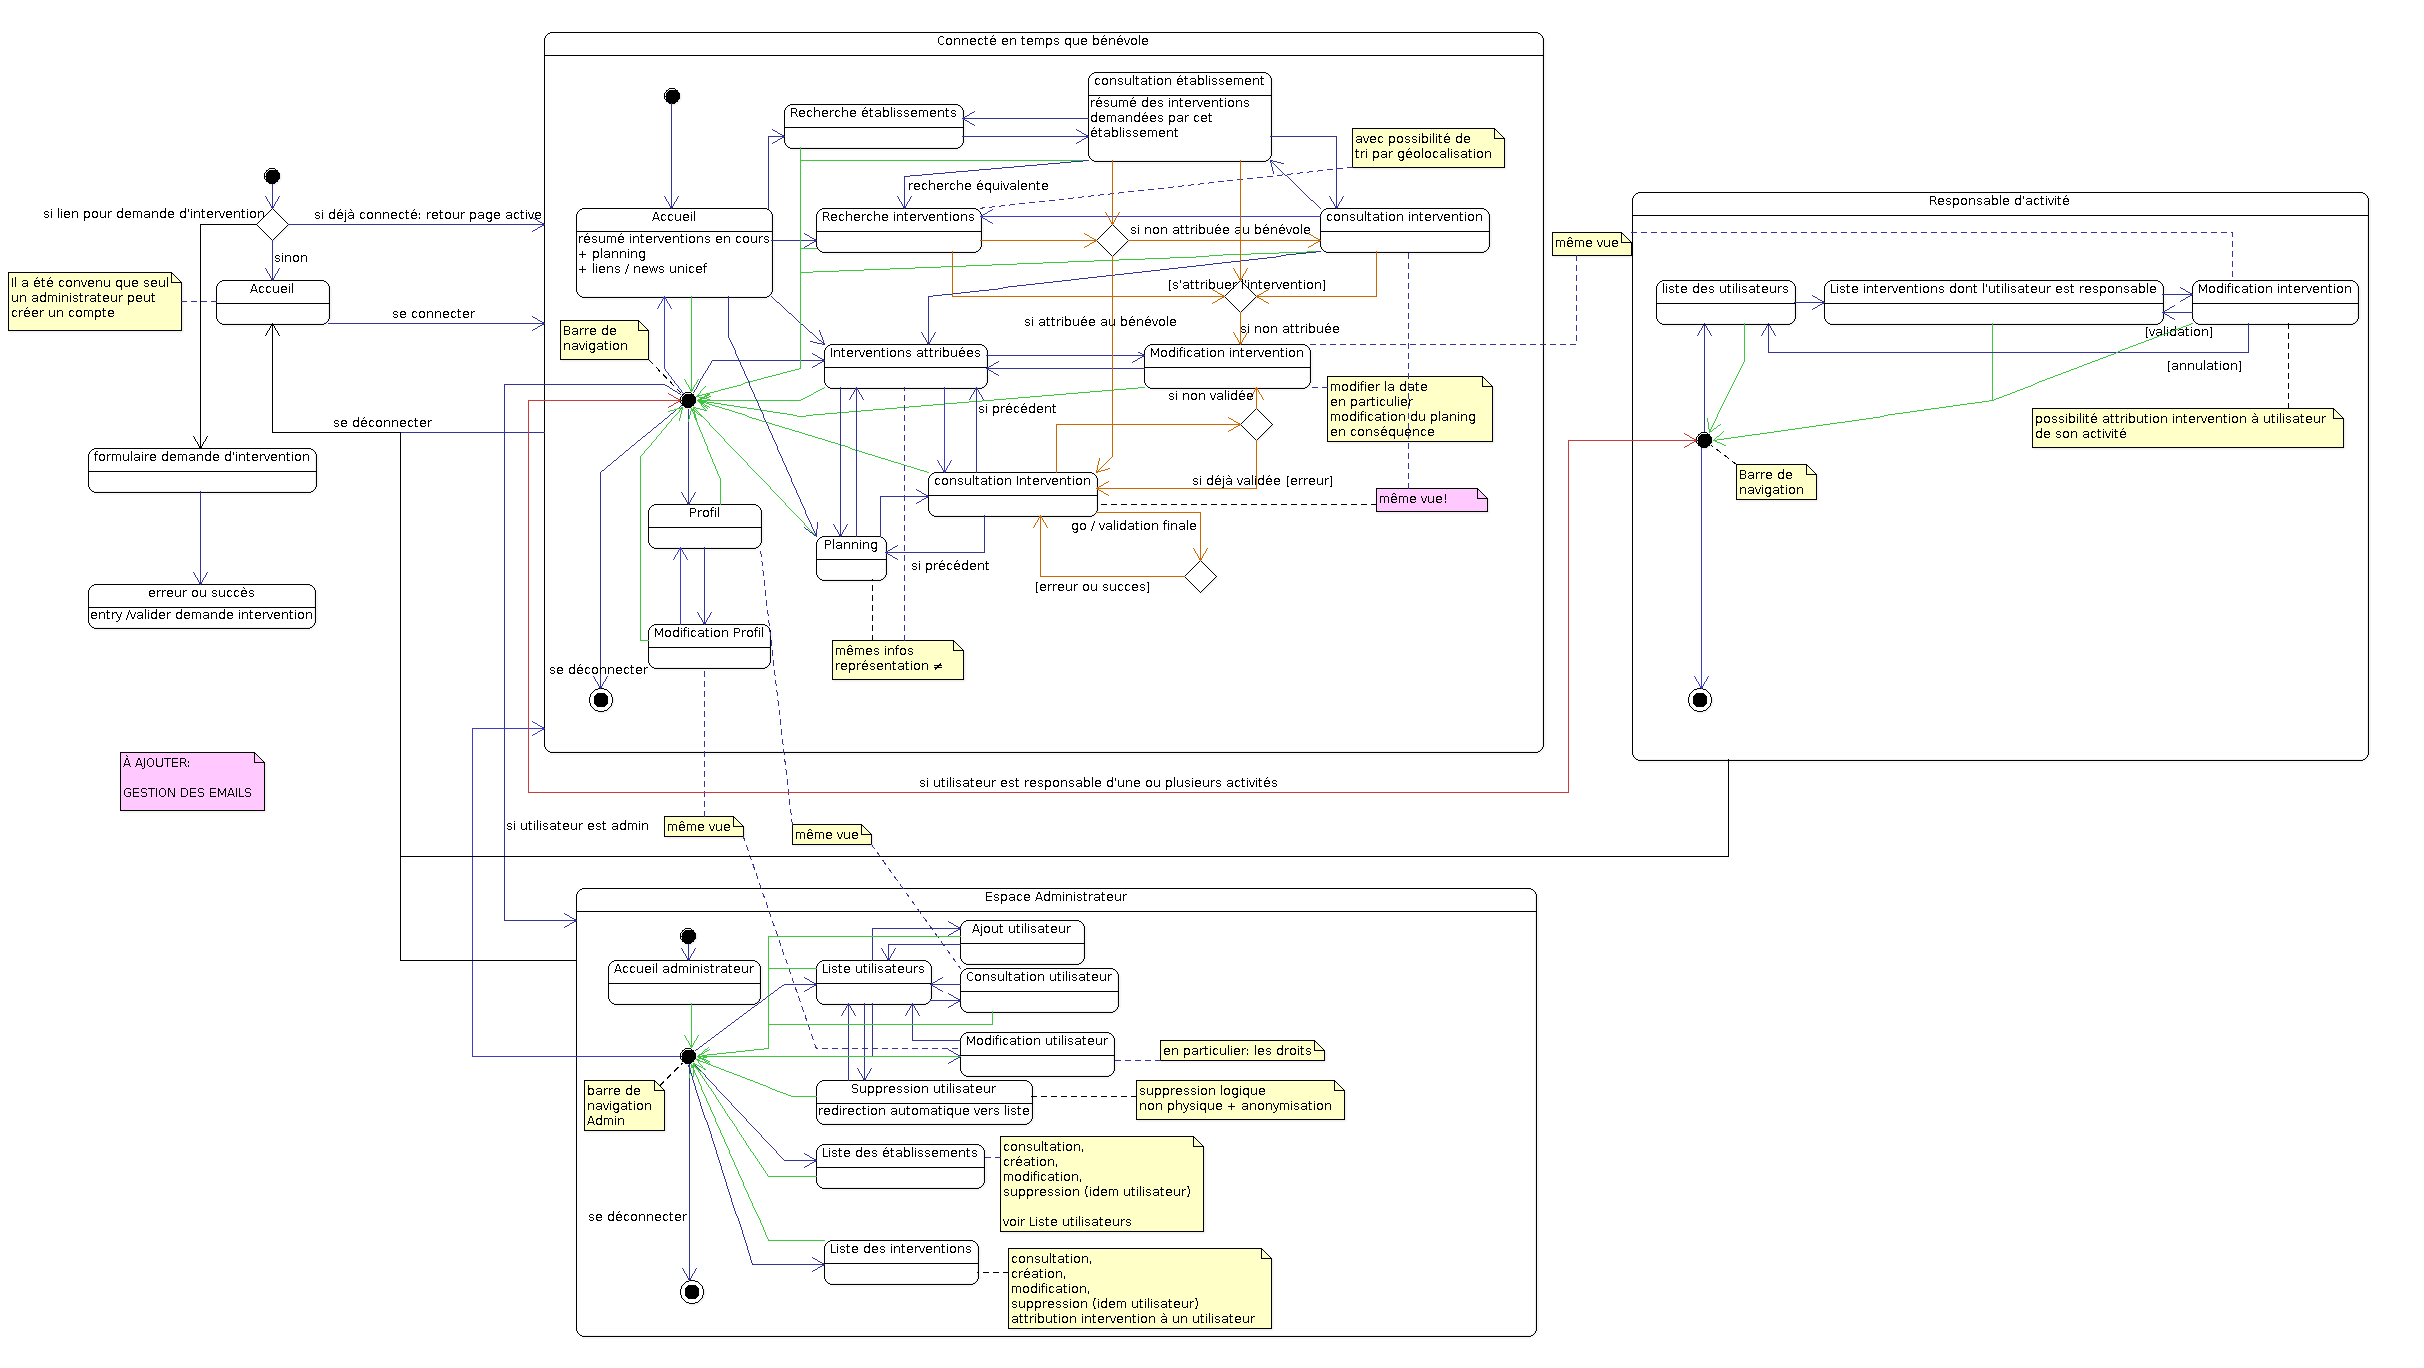
\includegraphics[scale=0.31, angle=90]{images/diagrammeEtatsTransitions/carteDeNavigation.png}
	\caption{Carte de navigation}
	\label{carteDeNavigation}
\end{figure}

\begin{appendix}
\part*{Annexes}
\addcontentsline{toc}{part}{Annexes}
\listoffigures
\addcontentsline{toc}{chapter}{Table des figures}
	 
\listoftables
\addcontentsline{toc}{chapter}{Liste des tableaux}
\end{appendix}
\pageQuatriemeCouverture

\end{document}
